\documentclass[a4paper]{report}

%%% Кодировки и шрифты %%%
\usepackage{cmap}						% Улучшенный поиск русских слов в полученном pdf-файле
\usepackage[T2A]{fontenc}				% Поддержка русских букв
\usepackage[utf8]{inputenc}				% Кодировка utf8
\usepackage[english, russian]{babel}	% Языки: русский, английский
%\usepackage{pscyr}						% Красивые русские шрифты
\usepackage[14pt]{extsizes}

\usepackage{listings}

%%% Математические пакеты %%%
\usepackage{amsthm,amsfonts,amsmath,amssymb,amscd} % Математические дополнения от AMS

%%% Оформление абзацев %%%
\usepackage{indentfirst} % Красная строка

%%% Цвета %%%
\usepackage[usenames]{color}
\usepackage{color}
\usepackage{colortbl}

%%% Библиография %%%
\usepackage{cite} % Красивые ссылки на литературу

%%% Гиперссылки %%%
\usepackage[linktocpage=true,plainpages=false,pdfpagelabels=false]{hyperref}

%%% Изображения %%%
\usepackage{graphicx} % Подключаем пакет работы с графикой

%%%%%%%%%%%%%%%%%%%%%%%%%%%%%%%%%%%%%%%%%
\begin{document}
\title{Лабораторная работа}
\author{Мельников А.О., Никифоров А.А.}
\date{Декабрь 2016}
\maketitle

Для функций, указанных в вариантах, посчитать две итерации алгоритма вычисления оптимального значения методом наискорейшего спуска (steepest descent) при
учете начального приближения ${{\bf x}_0 = [1\ 1]^T}$, вычислить тип оптимальной точки (минимум, максимум, глобальный минимум, глобальный максимум, седло),
вычислить значение оптимальной точки

Варианты:
\begin{enumerate}
    \item ${F({\bf x}) = \frac{7}{2}x_1^2 - 6 x_{1} x_{2} - x_2^2}$
    \item ${F({\bf x}) = 5x_1^2 -6x_1x_2 +5x_2^2 + 4x_1 +4x_2}$
    \item ${F({\bf x}) = \frac{9}{2}x_1^2 - 2x_1x_2 + 3x_2^2 + 2x_1 - x_2}$
    \item ${F({\bf x}) = -\frac{1}{2}(7x_1^2 + 12x_1x_2 - 2x_2^2)}$
    \item ${F({\bf x}) = x_1^2 + x_1x_2 + x_2^2 + 3x_1 + 3_2}$
    \item ${F({\bf x}) = \frac{1}{2}x_1^2 - 3x_1x_2 + 0.5x_2^2 - 4x_1 + 4x_2}$
    \item ${F({\bf x}) = \frac{1}{2}x_1^2 - 2x_1x_2 + 2x_2^2 + x_1 - 2x_2}$
    \item ${F({\bf x}) = \frac{3}{2}x_1^2 + 2x_1x_2 + 4x_1 + 4x_2}$
    \item ${F({\bf x}) = -\frac{3}{2}x_1^2 + 4x_1x_2 + 1.5x_2^2 + 5x_1}$
    \item ${F({\bf x}) = 2x_1^2 - 2x_1x_2 + 0.5x_2^2 + x_1 + x_2}$
\end{enumerate}

Основные формулы.

Градиент:
\begin{eqnarray}
    \nabla F({\bf x}) = \left[\frac{\partial}{\partial x_1}F({\bf x})\ \frac{\partial}{\partial x_2}F({\bf x})\ ...\ \frac{\partial}{\partial x_n}F({\bf x})\right]^T
\end{eqnarray}

Матрица Гессе:
\begin{eqnarray}
    \nabla^2 F({\bf x}) = 
    \left[
    \begin{matrix}
        \frac{\partial^2}{\partial x_1^2}F({\bf x}) & ... & \frac{\partial^2}{\partial x_1 ... \partial x_n}F({\bf x} \\
        \frac{\partial^2}{\partial x_1 ... \partial x_n}F({\bf x}) & ... & \frac{\partial^2}{\partial x_n^2}F({\bf x})
    \end{matrix}
    \right]
\end{eqnarray}

Метод наискорейшего спуска:
\begin{eqnarray}
    {\bf x_{k+1}} = {\bf x_k} - \alpha {\bf g_k} \\
    \alpha < \frac{2}{\lambda_{max}} \\
    {\bf g_k} = \nabla F({\bf x}) \vert_{\bf x=x_k}
\end{eqnarray}

Пример решения.

\begin{enumerate}
    \item Вычисление градиента функции:
        \begin{eqnarray}
            \nabla F({\bf x}) =
            \left[
                \begin{matrix}
                    7x_1-6x_2 \\
                    -6x_1-2x_2
                \end{matrix}
            \right]
        \end{eqnarray}

    \item Вычисление матрицы Гессе:
        \begin{eqnarray}
            \nabla^2 F({\bf x}) = \left[
                \begin{matrix}
                    7 & -6 \\
                    -6 & -2
                \end{matrix}
            \right]
        \end{eqnarray}

    \item Вычисление собственных значений матрицы:
        \begin{eqnarray}
           \left| 
                \begin{matrix}
                    7 - \lambda & -6 \\
                    -6 & -2 - \lambda
                \end{matrix}
           \right| = \lambda^2 - 5\lambda - 50 \\
           \lambda_1 = -5 \ \lambda_2 = 10
        \end{eqnarray}

        Собственные числа имеют разный знак - оптимальная точка имеет форму седла (saddle point).

    \item Вычисление предельного значения коэфициента спуска ${\alpha}$:
        \begin{eqnarray}
            \alpha < \frac{2}{\lambda_{max}} = \frac{2}{10} = \frac{1}{5}
        \end{eqnarray}

    \item Вычисление точки минимума/максимума
        \begin{eqnarray}
           \left[
                \begin{matrix}
                    7  & -6 \\
                    -6 & -2
                \end{matrix}
           \right]
           {\bf x}=
           \left[
                \begin{matrix}
                0 \\
                0
                \end{matrix}
           \right]
        \end{eqnarray}
    Следовательно:
        \begin{eqnarray}
           {\bf x}=
           \left[
                \begin{matrix}
                0 \\
                0
                \end{matrix}
           \right]
        \end{eqnarray}
    \item Выбор параметра ${\alpha}$: возьмем значение ${0.1}$ для простоты вычисления.

    \item Вычисление первого шага алгоритма:
        \begin{eqnarray}
            {\bf g_0} = \nabla F({\bf x})\left|_{\bf x=x_0}\right. =
            \left[
                \begin{matrix}
                    7*1 - 6*1 \\
                    -6*1 -2*1
                \end{matrix}
            \right]
            =
            \left[
                \begin{matrix}
                    1 \\
                   -8 
                \end{matrix}
            \right]
        \end{eqnarray}

        \begin{eqnarray}
            {\bf x_1} = {\bf _0} - \alpha {\bf g_0} = 
                \left[
                \begin{matrix}
                    1 \\
                    1
                \end{matrix}
                \right]
                - 0.1
                \left[
                \begin{matrix}
                    1 \\
                    -8
                \end{matrix}
                \right]
                =
                \left[
                \begin{matrix}
                    9 \\
                    1.8 
                \end{matrix}
                \right]
        \end{eqnarray}

    \item Вычисление второго шага алгоритма (значение ${\bf g_1}$ вычисляется так же как значение ${\bf g_0}$, только для вектора ${\bf x_1}$):
        \begin{eqnarray}
            {\bf x_2} = {\bf x_1} - \alpha {\bf g_1} = 
                \left[
                \begin{matrix}
                    0.9 \\
                    1.8
                \end{matrix}
                \right]
                - 0.1
                \left[
                \begin{matrix}
                    -4.5 \\
                    -9
                \end{matrix}
                \right]
                =
                \left[
                \begin{matrix}
                    1.35 \\
                    2.7 
                \end{matrix}
                \right]
        \end{eqnarray}
    
    \item Реализация алгиритма на ПЭВМ, демонстрация результатов (поверхности функции, график контуров).
    \begin{figure}[h]
        \center\scalebox{1}{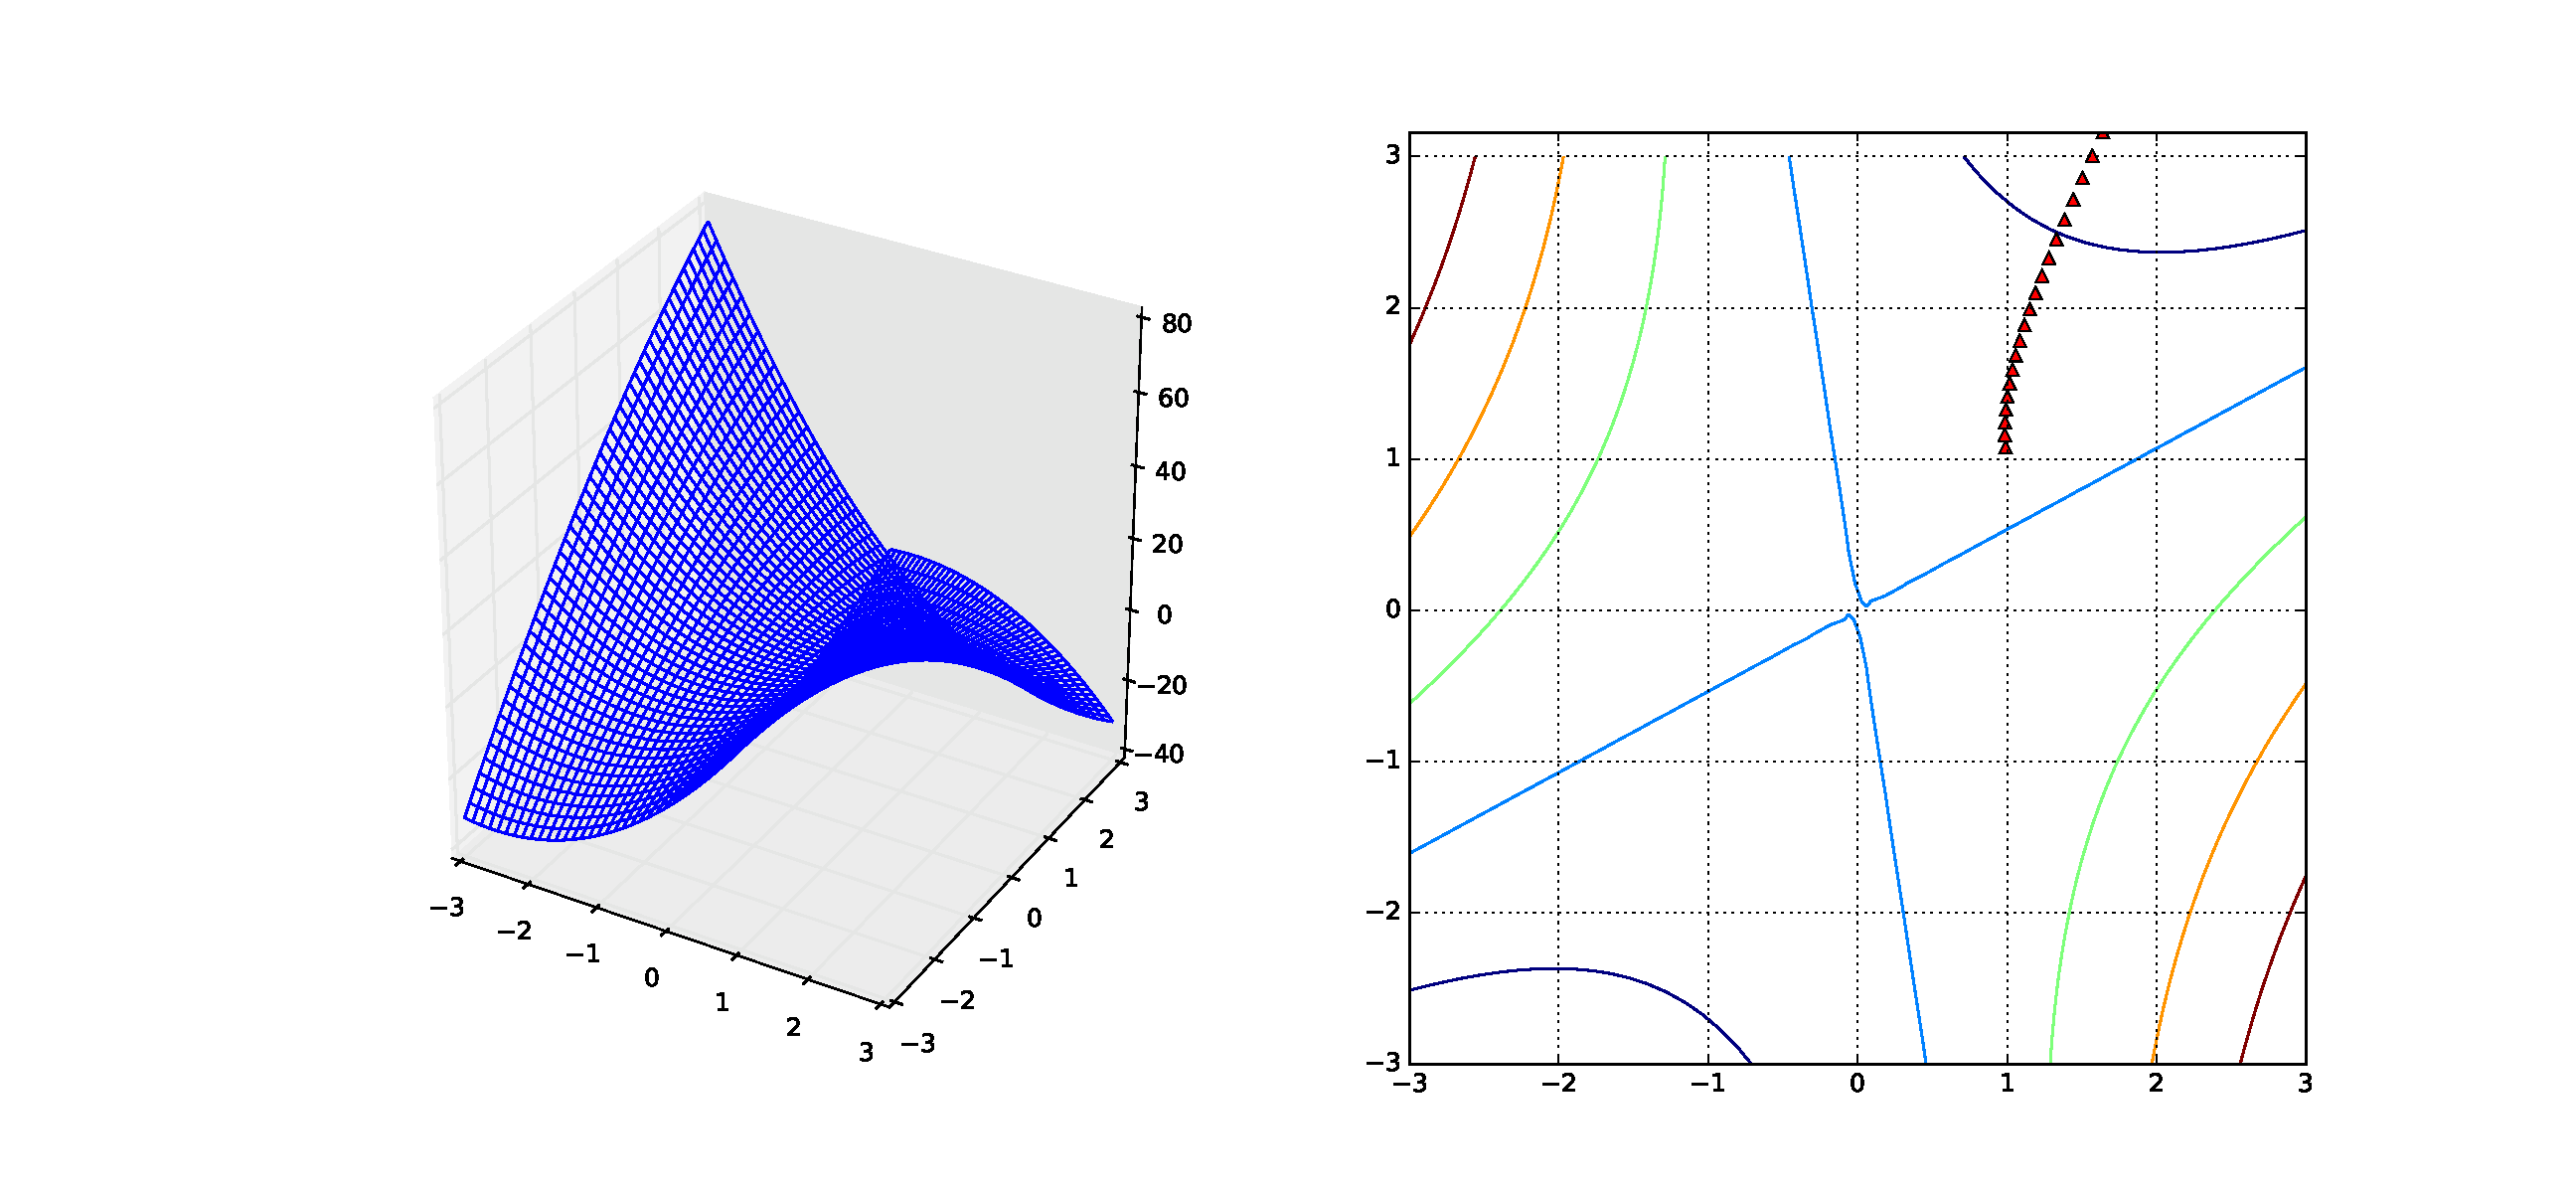
\includegraphics[width=1\linewidth]{figure_1}}
        \caption{Поверхность и график контуров} 
        \label{pic:graph}
    \end{figure}

    Как видно на графике, функция имеет седло в точке (0, 0)
\end{enumerate}

Литература:
\begin{enumerate}
    \item Gilbert Strang. Calculus (бесплатный доступ на сайте \href{http://ocw.mit.edu/ans7870/resources/Strang/Edited/Calculus/Calculus.pdf}{MIT OCW})
    \item Martin Hagan., et al Neural Network Design (2nd Edition) (бесплатный доступ на сайте \href{http://hagan.okstate.edu/nnd.html}{Martin Hagan})
\end{enumerate}

Исходный код на Python (требуются библиотеки matplot и numpy):
\lstset{language=Python,texcl=true}
\lstinputlisting[language=Python]{example.py}

\end{document}
